\begin{figure}%
	\centering%
	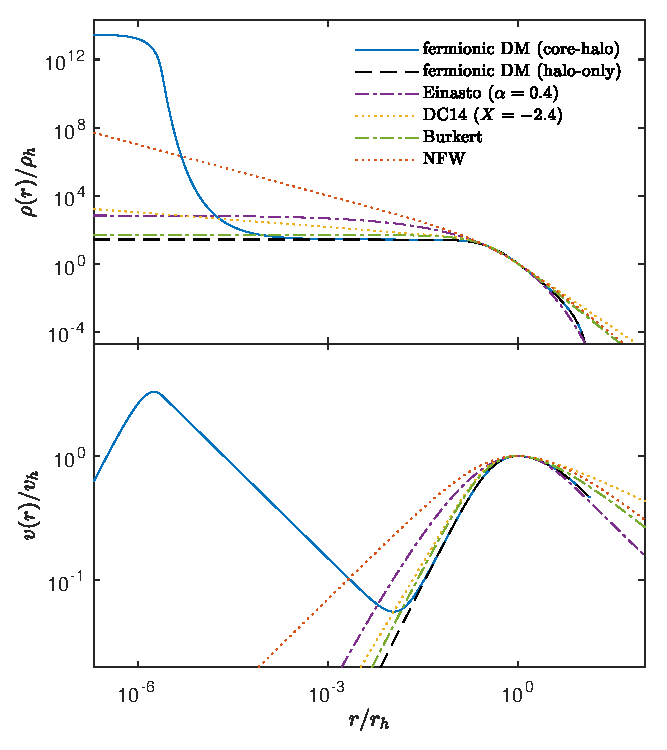
\includegraphics[width=\hsize]{\ROOTPATH/fig.pdf}
	\caption{Fermionic model predictions of the surface density for disk galaxies from the SPARC data-set. The blue region indicates the delimited area by the $3\sigma$ error bars of all the data points used in \citet{2009MNRAS.397.1169D}. The absolute magnitude was taken from the Carnegie-Irvine Galaxy Survey \citep{2011ApJS..197...21H}, providing nine overlapping galaxies (blue and green circles). The full sample (gray bars) and a sub-sample (green bars), including only non-isothermal solutions with $W_p < 10$, are shown as histograms, both following approximately a Gaussian distribution.}%
	\label{fig:SPARC:Donato}%
\end{figure}